\documentclass[tikz, border=2pt]{standalone}
\usetikzlibrary{shapes.geometric, arrows, positioning}
\usetikzlibrary{backgrounds}


\tikzset{
  box/.style  = {draw,rectangle, minimum width=5cm, minimum height=1.2cm, text centered, text width=5cm, font=\Large},
  myarrow/.style = {line width=2mm, draw=blue, -triangle 60, postaction={draw, line width=4mm, shorten >=6mm, -}}
}


\begin{document}
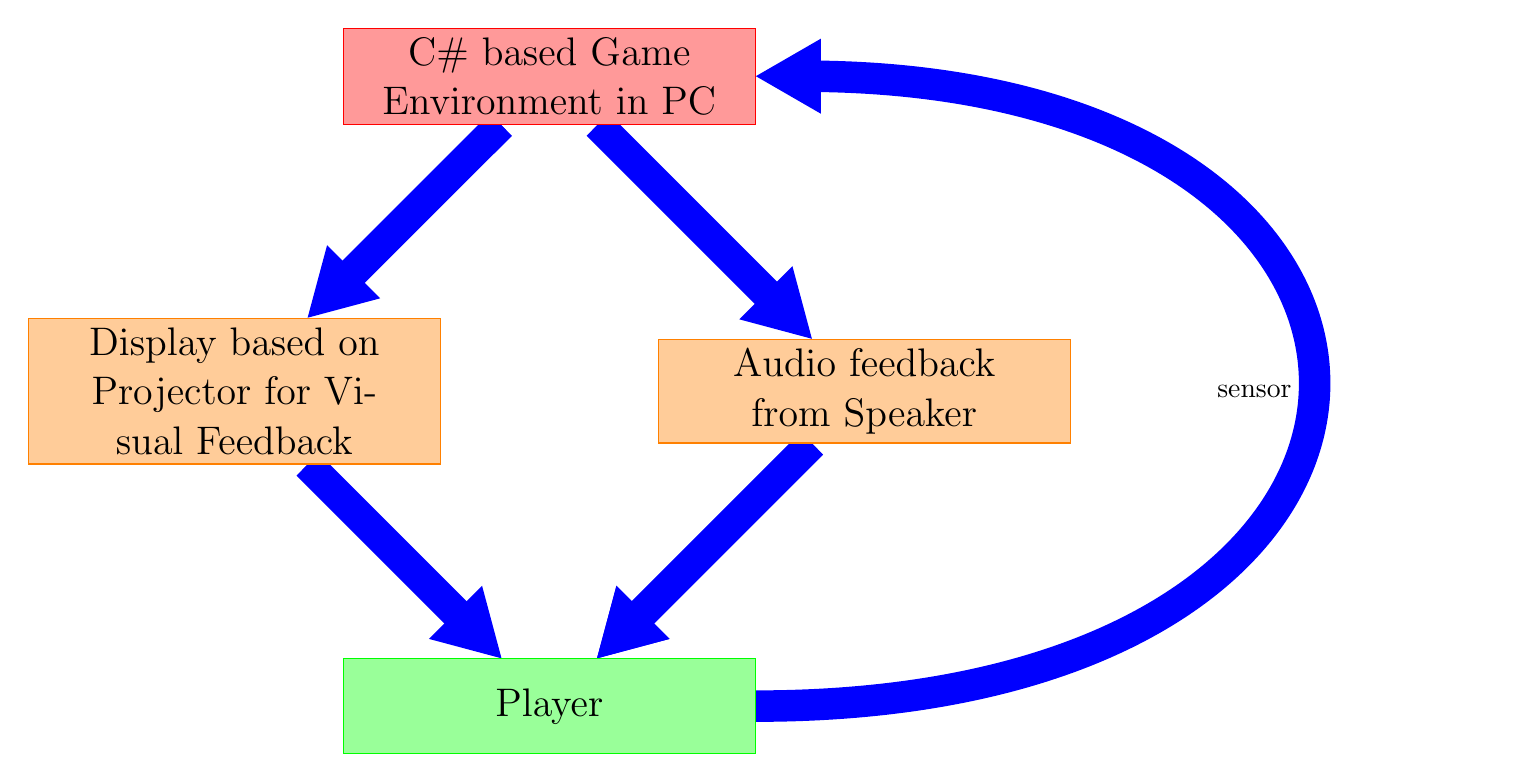
\begin{tikzpicture}[node distance=4cm]
    \node (n00) [box, draw=red, fill=red!40] {C\# based Game Environment in PC};
    \node (n10) [box, draw=orange, fill=orange!40, below of=n00, xshift=-4cm] {Display based on Projector for Visual Feedback};
    \node (n11) [box, draw=orange, fill=orange!40, below of=n00, xshift=+4cm] {Audio feedback from Speaker};
    \node (n20) [box, draw=green, fill=green!40, below of=n10, xshift=+4cm] {Player};

    \begin{scope}[on background layer]
        \draw [myarrow] (n00) -- (n10);
        \draw [myarrow] (n00) -- (n11);
        \draw [myarrow] (n10) -- (n20);
        \draw [myarrow] (n11) -- (n20);
        \draw [myarrow] (n11) -- (n20);
        \draw [myarrow] (n20.east)  to [out=0, in=0, looseness=3] node[left]{sensor} (n00.east);
    \end{scope}

\end{tikzpicture}
\end{document}
